% Chapter 2
\chapter{The Mechanics of C++: from Source Code to a Running Program}

\section{Introduction and objectives}

\section{The compilation process}

\section{Header files and source files}

\lstinputpath{../../src/chapter_2}

\lstinputlisting[
	caption={Header files containing declarations of functions},
	label=Inequalities.hpp,
]{Inequalities.hpp}

\lstinputlisting[
	caption={Code files containing bodies of functions},
	label=Inequalities.cpp,
]{Inequalities.cpp}

\lstinputlisting[
	caption={Math program (Console-based) to test Max and Min functions.},
	label=TestInequalities.cpp,
]{TestInequalities.cpp}

\lstinputlisting[
	language=bash,
	caption={Output of \texttt{TestInequalities.cpp}.},
	label=TestInequalities.txt,
]{TestInequalities.txt}

\section{Creating classes and using their objects}

\begin{lstlisting}
#include <string>	// Standard string class in C++
using namespace std:
\end{lstlisting}

\begin{lstlisting}
#include "DatasimDate.hpp"	// Dates and other useful stuff
#include "Person.hpp"	// Interface functions for Person
\end{lstlisting}

\begin{figure}[ht!]
	\centering
	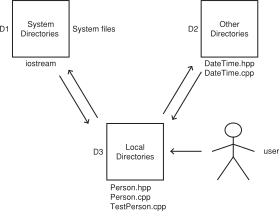
\includegraphics[width=0.4\paperwidth]{./../img/figure2_1}
	\caption{Directory structure for project.}
\end{figure}

\lstinputlisting[
	caption={Hello World class.},
	label=Person.hpp,
]{Person.hpp}

\lstinputlisting[
	caption={Hello World class.},
	label=Person.cpp,
]{Person.cpp}

\lstinputlisting[
	caption={Hello World Testing the first C++ class.},
	label=TestPerson.cpp,
]{TestPerson.cpp}

\lstinputlisting[
	caption={Output of \texttt{TestPerson.cpp}.},
	label=TestPerson.txt,
]{TestPerson.txt}

\section{Template classes and template functions}

\lstinputlisting[
	caption={Header file containing declarations of functions.},
	label=GenericInequalities.hpp,
]{GenericInequalities.hpp}

\lstinputlisting[
	caption={Code file containing declarations of functions.},
	label=GenericInequalities.cpp,
]{GenericInequalities.cpp}

\lstinputlisting[
	caption={Main program (Console-based) to test Max and Min functions.},
	label=TestGenericInequalities.cpp,
]{TestGenericInequalities.cpp}

\section{Kinds of errors}



\subsection{Compiler errors}

\subsection{Linker errors}

\begin{lstlisting}
int age(); // NO "const" in this declaration
\end{lstlisting}

\begin{lstlisting}
int Person::age() const
{
	return int( double(DatasimDate() - dob) / 365.0);
}
\end{lstlisting}

\lstinputlisting[
	caption={Simple stuff for converting built-in types to strings.},
	label=TestConversions.cpp,
]{TestConversions.cpp}

\begin{lstlisting}
#include <string>
#include <cstddef>

stdd::string getString(long j)
{
	char str[200];
	sprintf(str, "%d", j);
	std::string result(str);
	
	return result;
}

stdd::string getString(int j)
{
	char str[200];
	sprintf(str, "%d", j);
	std::string result(str);

	return result;
}

stdd::string getString(size_t j)
{
	char str[200];
	sprintf(str, "%d", j);
	std::string result(str);

	return result;
}
\end{lstlisting}

\subsection{Run-time errors}

\section{The struct concept}

\section{Useful data conversion routines}

\begin{lstlisting}
// Hard-coded example for starters
std::stringstream s;
s << myDouble;
std::string result = s.str();
std::cout << "String value is: " << result << std::endl;
\end{lstlisting}

\begin{lstlisting}
template <typename T>
	std::string getString(const T& value)
{
	stringstream s;
	s << value;
	return s.str();
}
\end{lstlisting}

\section{Summary and conclusions}

\section{Exercises and projects}